\documentclass{report}
\usepackage{listings}
\usepackage{hyperref}
\usepackage{tikz}
\usetikzlibrary{shapes.geometric, arrows, positioning}
\tikzstyle{process} = [rectangle, minimum width=3cm, minimum height=1cm, text centered, text width=6cm, draw=black]
\tikzstyle{arrow} = [thick,->,>=stealth]

\begin{document}

\title{Tastydoc: a documentation tool for dotty using Tasty files}
\author{Bryan Abate
\\\\\small{Supervised by Aleksander Boruch-Gruszecki}}

\maketitle

\begin{abstract}
The current documentation tool (Dottydoc) relies on compiler internals and low-level code. The tool introduced here aims to build a program not dependant on compiler internals but instead use Tasty files which are output when a Scala program is compiled.

It also aims at providing a tool with fewer bugs, more features and which is more easily maintainable.

The output documentation files are in Markdown instead of the commonly used HTML.
\end{abstract}

\tableofcontents

\chapter{Introduction}

A documentation tool is a program generating information (often in the form of HTML files) about projects, it usually includes method signatures, user-written documentation, link to other pages of the documentation, etc.
In Dotty, the current tool for generating Scala project documentation is called Dottydoc. The tool introduced here, called Tastydoc, aims to improve on Dottydoc and replace it.

Tastydoc makes use of TASTy files. These files are output when a program is compiled, they contain information about the source code of a program. Tastydoc consumes such files to extract information about the code, that way it is completely independent of the compiler and can be used on its own.
The tool tries to be as close as possible to the structure proposed in Dottydoc so that it can reuse some partial portions of its code with minor modifications.
Although documentation is often output as HTML files, here we choose to output Markdown files for reasons we detail further in the report.

The tool was developed with a few goals in mind. It should be independent of the compiler, hence the use of TASTy files. It should produce humanly consumable files, hence the choice of Markdown as an output. It should have as many features as Dottydoc and be easily maintainable.

The report is organized in the following structure: First, we will talk about the features of the tool, then give a high-level and a low-level architectural description. Dottydoc and Tastydoc will then be compared. We will finally talk about the problems encountered during the development and further work.

\chapter{Features}
We will list here the most important features of Tastydoc.

\paragraph{Accessible information}
The tool has knowledge of the full signature of entities meaning it is aware of annotations, modifiers (including scope modifiers), parameters, type parameters, and return types.
For classes, traits, and objects the following are also available: members, parents, constructors, known subclasses and companion.
Packages know all their members as long as corresponding TASTy files were passed as arguments to the tool.

User-written documentation, including individual access to defined @ (except \texttt{@usecase}), is present as well. Two syntaxes are supported, which is the old Scaladoc Wiki-style syntax as well as Dottydoc Markdown syntax. Linking to entities (classes, methods, etc.) is possible inside the user documentation in the Wiki-style syntax using the notation like \texttt{[[scala.foo.bar]]}.

\paragraph{TASTy}
The tool relies on consuming TASTy files and is hence independent to the compiler.

\paragraph{Linking}
Tastydoc is able to produce links to types defined outside of the current TASTy files (as well as the one inside the file). This is particularly useful for linking to parameters and return types, companions, and parents.

\paragraph{Output}
The tool produces Markdown documentation files that are easy to modify and read.

\chapter{Architecture}
\section{High-level architectural descriptions}
\subsection{TASTy}
TASTy is a data format aimed at serializing compiler information about code. Dotty produces these files for each class, object without companion class or trait, trait and package if it contains something else than classes, traits or objects. From its nature, it should be perfect to extract information from.
This is done through the use of the reflect API and making a class extanding \texttt{TastyConsumer}\footnote{\texttt{scala/tasty/file/TastyConsumer.scala}}.

\subsection{High-level API}
The tool offers an easy to use interface (called Representation, see \autoref{sec:representation}) to access all the information about an entity for anyone willing to write their own documentation tool without worrying to consume TASTy files.

\subsection{Reuse of Dottydoc intermediate representation}
The intermediate structure (Representation) is similar do Dottydoc \texttt{Entity}\footnote{\texttt{dotty/tools/dottydoc/Entity.scala}} which allows for an easy reuse of part of Dottydoc code with minor modifications. Right now, the tool uses some code from Dottydoc for parsing user documentation. But we can think of using it to produce the same HTML files as does Dottydoc but without relying on compiler internals for example. Especially that Dottydoc already has a complex templating mechanism that allows attaching blog posts to documentation.

\subsection{Markdown}
Outputting Markdown instead of HTML has several advantages. It is easy to edit by hand, easily previewed, and users can easily add their own text or own file. A user could, for example, write a Markdown file and link it in the documentation of a class; or do the opposite link a documentation page in a Markdown file.

Markdown files can be easily uploaded to GitHub or GitLab, hence it would be extremely easy to upload documentation files along with the code of a project.

In addition to that lots of tools are available to consume Markdown files and output other formats such as HTML or PDF making Markdown a nice intermediate representation. From this we can imagine a pipeline like this:
\begin{center}
    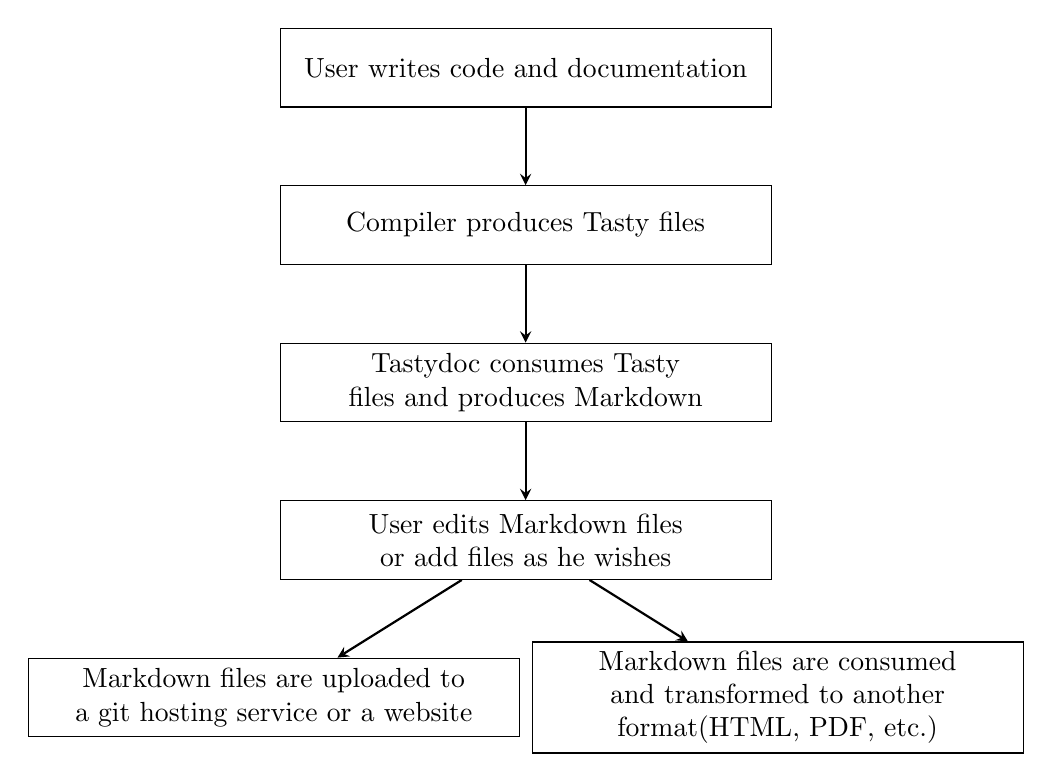
\begin{tikzpicture}[node distance=2cm]
        \node (write) [process] {User writes code and documentation};
        \node (compile) [process, below of=write] {Compiler produces Tasty files};
        \node (tool) [process, below of=compile] {Tastydoc consumes Tasty files and produces Markdown};
        \node (user) [process, below of=tool] {User edits Markdown files or add files as he wishes};
        \node (HTML) [process, below of=user, right of=user, xshift=1.2cm] {Markdown files are consumed and transformed to another format(HTML, PDF, etc.)};
        \node (upload) [process, below of=user, left of=user, xshift=-1.2cm] {Markdown files are uploaded to a git hosting service or a website};
    
        \draw [arrow] (write) -- (compile);
        \draw [arrow] (compile) -- (tool);
        \draw [arrow] (tool) -- (user);
        \draw [arrow] (user) -- (HTML);
        \draw [arrow] (user) -- (upload);
    \end{tikzpicture}
\end{center}

\section{Low-level architecture}
\subsection{TastyExtractor}
File: \texttt{dotty/tastydoc/TastyExtractor.scala}

A trait containing useful methods for extracting information from the reflect API.

\subsection{References}
File: \texttt{dotty/tastydoc/references.scala}

Object containing case classes. References are classes containing information about a specific type to be able to link to its documentation file later on. This is inspired from Dottydoc Reference\footnote{dotty/tools/dottydoc/model/references.scala}. There exists a reference for all the existing special types such as "or type". Referencing a user-defined type (such as a class or a type alias) is done using a label (the name of the type, like "String") and a path (the full path in which it is defined, like "/scala/Predef/").

\subsection{TastyTypeConverter}
File: \texttt{dotty/tastydoc/TastyTypeConverter.scala}

Trait containing methods for converting from Reflect types to References.

\subsection{Representation}
\label{sec:representation}
File: \texttt{dotty/tastydoc/representations.scala}

Object implementing both \texttt{TastyExtractor} and \texttt{TastyTypeConverter}

A Representation contains all the information of a specific entity. The logic is as follows: there exist different trait such as \texttt{Modifiers} or \texttt{Members} and classes which implement those traits. This logic is inspired by dotty-doc Entities\footnote{\texttt{dotty/tools/dottydoc/Entity.scala}}.

A Representation take a reflect class such as \texttt{reflect.ClassDef} and extract every information from it using mostly \texttt{TastyExtractor} functions while converting types to References using \texttt{TastyTypeConverter} functions.

Representations can then be easily used for printing, their content is self-explanatory and no knowledge of Tasty is required to use them as the implementation is not exposed from the outside.

We give below the existing Representation, a quick description and their signature (without parameters).
\begin{itemize}
    \item \texttt{PackageRepresentation} For packages
\begin{lstlisting}[language=scala]
class PackageRepresentation(...)
extends Representation with Members
\end{lstlisting}
    \item \texttt{ImportRepresentation} For imports, never used in the tool
\begin{lstlisting}[language=scala]
class ImportRepresentation(...)
extends Representation
\end{lstlisting}
    \item \texttt{ClassRepresentation} For classes, objects and traits, including case classes and case objects.
\begin{lstlisting}[language=scala]
class ClassRepresentation(...)
extends Representation with Members
with Parents with Modifiers with Companion
with Constructors with TypeParams
\end{lstlisting}
    \item \texttt{DefRepresentation} For defs
\begin{lstlisting}[language=scala]
class DefRepresentation(...)
extends Representation with Modifiers
with TypeParams with MultipleParamList
with ReturnValue
\end{lstlisting}
    \item \texttt{ValRepresentation} For vals and vars
\begin{lstlisting}[language=scala]
class ValRepresentation(...)
extends Representation with Modifiers
with ReturnValue
\end{lstlisting}
    \item \texttt{TypeRepresentation} For type alias
\begin{lstlisting}[language=scala]
class TypeRepresentation(...)
extends Representation with Modifiers
with TypeParams 
\end{lstlisting}
    \item \texttt{EmulatedPackageRepresentation} This Representation is a trick for regrouping every PackageRepresentation of the same package under the same Representation. Indeed the way Tasty works is that for each class or trait it will output a Tasty file and the top of \texttt{reflect.Tree} is a\texttt{reflect.PackageClause}, hence when converting multiple classes of the same package, there will be multiple \texttt{PackageRepresentation} of the same package. In the point of view of usability, this is not the best and this Representation is here to counter this problem. When using an \texttt{EmulatedPackageRepresentation}, for the user it looks like he is using a \texttt{PackageRepresentation} containing all the members of the package.
\end{itemize}

\subsection{DocPrinter}
File: \texttt{dotty/tastydoc/DocPrinter.scala}

Object with functions for formatting Representations and References to Markdown and writing them to files. Basically, handle all the formatting and printing logic of the tool.

\subsection{mdscala}
File: \texttt{dotty/tastydoc/mdscala.scala}

Object with helper functions for outputting markdown. Unfortunately, it does not handle escaping as it is a non-trivial task and would have required a significant amount of time. (See \autoref{sec:problems})

\subsection{TastyDocConsumer}
File: \texttt{dotty/tastydoc/TastyDocConsumer.scala}

Extends TastyConsumer and consumes TASTy files to produce Representations. It needs a \texttt{mutable.HashMap[String, EmulatedPackageRepresentation]} as parameters for adding every new seen package to the map. This is some required behavior for two things: linking inside user documentation and a data structure for storing converted Representations.
\subsection{Main}
File: \texttt{dotty/tastydoc/Main.scala}

Manages the workflow (see \autoref{sec:workflow}).

Command line arguments are:
\begin{itemize}
    \item \textbf{-syntax} \{\textit{wiki} or \textit{markdown}\} Syntax to use for user documentation parsing
    \item \textbf{-packagestolink} \{\textit{regex1 regex2 ...}\} Regexes to specify which packages should be linked when formatting References
    \item \textbf{-classpath} \{\textit{URI}\} Extra classpath for input files
    \item \textbf{-i} \{\textit{file1 file2 ...}\} Tasty files
\end{itemize}

\subsection{User documentation parsing}
Files are in the package \texttt{dotty.tastydoc.comment}.

These files are taken from Dottydoc (slightly modified to work with this architecture and output Markdown instead of HTML) and are responsible for parsing user-written documentation.

Note that it is using a library called flexmark-java\footnote{\url{https://github.com/vsch/flexmark-java}} for parsing user documentation written in Markdown.

\section{Workflow}
\label{sec:workflow}
Main workflow is as follows:

\begin{center}
    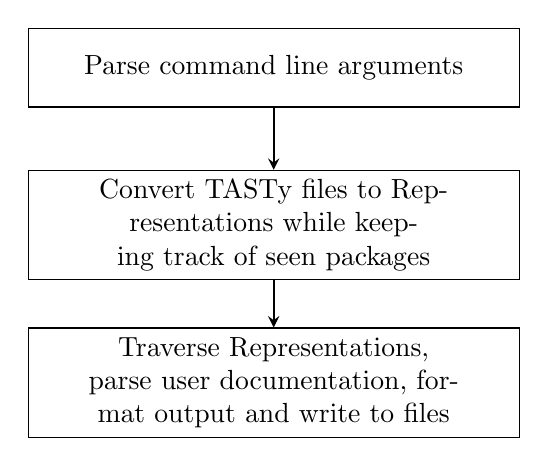
\begin{tikzpicture}[node distance=2cm]
        \node (parse) [process] {Parse command line arguments};
        \node (convert) [process, below of=parse] {Convert TASTy files to Representations while keeping track of seen packages};
        \node (output) [process, below of=convert] {Traverse Representations, parse user documentation, format output and write to files};
    
        \draw [arrow] (parse) -- (convert);
        \draw [arrow] (convert) -- (output);
    \end{tikzpicture}
\end{center}

As we can see, parsing user documentation is only done after converting to Representation. Indeed to be able to link methods, classes, etc. from user documentation we need to have converted everything to Representation first otherwise there is no way to know what is linked (a method? a class? an object?).
\chapter{Comparison between Dottydoc and Tastydoc}
Here we compare Dottydoc and Tastydoc in terms of features, bugs, and output.

\paragraph{Compiler internals}
Dottydoc heavily relies on compiler internals and hence cannot be detached from it. Tastydoc relies on TASTy files and hence can be completely moved apart from the compiler and can be distributed as a separate tool.

Dottydoc relies on low-level and complex code which makes it very hard to maintain or add features where Tastydoc relies on the comprehensive Reflect API while trying to be as clear and as maintainable as possible.

\paragraph{Scope modifiers}
Dottydoc does not handle scope modifiers (such as \texttt{private[this]}) where Tastydoc does.

\paragraph{Output}
Dottydoc outputs HTML/CSS with a preformatted template and offers no way to customize anything. Also, HTML/CSS force the user to host it on a website where Markdown can simply be viewed on an online git repository without further tasks. Tastydoc counters this problem by outputting Markdown.

\paragraph{Not maintained}
Dottydoc is not maintained and hence does not follow the evolution in Master. This opens to bugs for example it does not take care of colors in the \texttt{show} method and it results in faulty type or method output like \texttt{[31m2L[0m}\footnote{\url{https://dotty.epfl.ch/api/dotty/runtime/LazyVals$.html}}. Classes often show to be extending Object instead of their superclass because Object is given first when asking for the parents list to the compiler, example\footnote{\url{https://dotty.epfl.ch/API/scala/Conversion.HTML}}:
\begin{lstlisting}[language=scala]
    abstract class Conversion [ -T, +U ]
    extends Object with Function1
\end{lstlisting}
Annotations which should not be displayed (like \texttt{@child}) are displayed and sometimes many times\footnote{\url{http://dotty.epfl.ch/api/scala/quoted/Expr.html}}.

\paragraph{Known subclasses}
Tastydoc keeps track of all seen subclasses of a class and links to their documentation files.

\chapter{Problems}
\label{sec:problems}
A few problems were encountered during the development, some could not be fixed for reasons detailed below.

\paragraph{Markdown escaping}
The output being in Markdown we need a library to create a Markdown AST and render it to text. The library also needs to escape the input, indeed, assume we have a String "\#", if we do not escape it, Markdown will interpret it as a header of level 1 and this is not the expected behavior. This is where we have a problem because no such library exists in Java or Scala and taking care of Markdown escaping would have been time-consuming and was not the main topic of this project.

\paragraph{Linking inside code blocks}
We use code blocks indicating we have a piece of code so that a signature is formatted and syntax highlighted. In these code blocks, we also want to be able to make links pointing to the documentation page of a type. Unfortunately, Markdown fenced code blocks do not allow to have links in them. To counter this problem we use HTML pre and code tag which are also understood by Markdown viewer but this causes two problems. First, it is not pure Markdown anymore and then we lose the language syntax highlight from Markdown fenced code blocks.

\paragraph{Section}
Markdown does not have "division" with classes like the \texttt{<div>} tag in HTML which could be useful to better structure the page into sections. This is, however, the philosophy of Markdown and is hence an expected feature.

\paragraph{IDs for linking}
If a single entity contains a type and a method definition with the same name (overloaded methods suffer from the same problem), the links we generate do not always point to the correct definition because it links to the first one appearing on the page. This is because most Markdown viewer does not understand user-specified id which could be useful for linking to specific things on the same page. Hence we do not use custom ids for linking in this project and only use automatically generated ids from headers.

To mitigate this problem, we first output types and then values so that when linking it links to the first one appearing in the page which would be a type and it is what we want in most cases. However, this does not solve the problem of linking to type parameters and of linking to overloaded methods.

\paragraph{Multi-level lists}
Flexmark-java Markdown parser does not understand when ordered and unordered lists are combined, they are parsed as 2 separate lists instead of a multi-level list. Basically, if we have:
\begin{enumerate}
    \item foo
    \begin{itemize}
        \item bar
    \end{itemize}
\end{enumerate}
It will be parsed as:
\begin{enumerate}
    \item foo
\end{enumerate}
\begin{itemize}
    \item bar
\end{itemize}

\chapter{Remaining work}
Although the project is near features complete. Some work needs to be done to perfect the tool.

\paragraph{Markdown escaping}
As seen in \autoref{sec:problems} we do not escape anything before outputting Markdown, this is a problem that needs to be addressed by making a library capable of making a Markdown AST and rendering it to text while escaping the input. This is not a trivial task as Markdown has a lot of different available syntaxes, especially when we extend Markdown with some features like tables.

\paragraph{Type Lambdas}
Type Lambdas are complex types to handle and convert to References, right now they are converted to constant References. This is not the expected behavior and the output is not the one we expect and no linking can be done this way. It is, however, acceptable for a first version as type lambdas do not appear that often.

\paragraph{User-documentation parsing}
User-documentation parsing lacks two features: supporting \texttt{@usecase} and supporting defined pieces of documenation with \texttt{@define name ...} and then referencing them with \texttt{\$name}\footnote{Example in \url{https://github.com/scala/scala/blob/v2.12.2/src/library/scala/collection/immutable/List.scala\#L73}}.

\paragraph{HTML/CSS}
Markdown files for documentation are good for all the reasons mentioned in this report but some people still want a good HTML/CSS documentation. The aim here would be to either take back what Dottydoc has and use it with our code, either build something new. The first case should be pretty straightforward as our intermediate representation looks very much alike Dottydoc. The biggest change would be for References as links are handled a bit differently in this tool.

\end{document}